\documentclass[a4paper, 12pt]{article}
\usepackage[utf8]{inputenc}
\usepackage{polski}
\usepackage[polish]{babel}
\usepackage{graphicx}
\usepackage{float}
\usepackage{inputenc}
\usepackage{enumitem}

\begin{document}
\begin{titlepage}
	\centering
	{\scshape\LARGE Politechnika Wrocławska \par}
	\vspace{1cm}
	{\scshape\Large Wydział Elektroniki\par}
	\vspace{1.5cm}
	{\huge\bfseries Internetowy sklep sportowy oparty o relacyjną bazę danych\par}
	\vspace{2cm}

	\begin{flushright}
	\Large Prowadzący zajęcia:\par
	\large Dr~inż. Robert Wójcik\\
	\end{flushright}

    \begin{flushleft}
	{\Large Autorzy:\par}
	{\large Tomasz Bartos - 209248\par}
	{\large Jakub Dymon - 200335\par}
	{\large Wiktor Gerstenstein - 209138\par}
	\end{flushleft}
	
	\begin{minipage}{0.6\textwidth}
	\begin{flushright}
	\Large Ocena:
	\end{flushright}
	\end{minipage}
	
	\vfill
	{\large Wrocław 2016\par}
\end{titlepage}

\tableofcontents
\pagenumbering{arabic}

\listoffigures
\cleardoublepage

\listoftables
\cleardoublepage

\section{Wstęp}
\subsection{Cel projektu}
Celem projektu jest zaprojektowanie systemu bazodanowego dla~internetowego sklepu sportowego oraz~implementacja aplikacji webowej umożliwiającej dokonywanie wybranych transakcji zarówno od~strony klienta jak~i~sprzedawcy.
\subsection{Zakres projektu}
System pozwala sprzedawcy na dodawanie towarów do~sklepu, wystawianie ich~do~sprzedaży, kontrolę ilości towaru dostępnej na~magazynie oraz~generowanie prostych raportów na~temat sprzedaży, natomiast kupujący ma~możliwość wyszukiwania towaru, zakupu i~listowania dokonanych zakupów oraz~statusu zamówienia. Aplikacja jest dostępna w~formie strony internetowej umieszczonej na~serwerze i~dostępnej po~zalogowaniu. Istnieje możliwość założenia konta w~dwóch wariantach:
\begin{itemize}
	\item Handlowca
	\item Klienta
\end{itemize}
Zależnie od rodzaju konta udostępniana jest określona wersja serwisu.
\section{Analiza wymagań}
\subsection{Opis działania i schemat logiczny systemu}
System jest zrealizowany w oparciu o relacyjną bazę danych MySQL~oraz interfejs dostępowy utworzony w~języku PHP. Operacje dostępowe oraz przetwarzanie danych odbywają się po stronie bazy danych, natomiast dla klienta udostępnione jest graficzne środowisko dostępowe umożliwiające wydawanie żądanych zapytań. Klient ma możliwość sprawdzenia wybranych zawartości tabel, modyfikacji danych oraz ich usuwawania. Wykonywanie poleceń w~systemie bazodanowym nie wymaga od użytkownika znajomości języka SQL.
Schemat logiczny systemu znajduje się na Rysunku \ref{fig:schematLogiczny}

\begin{figure}[H]
	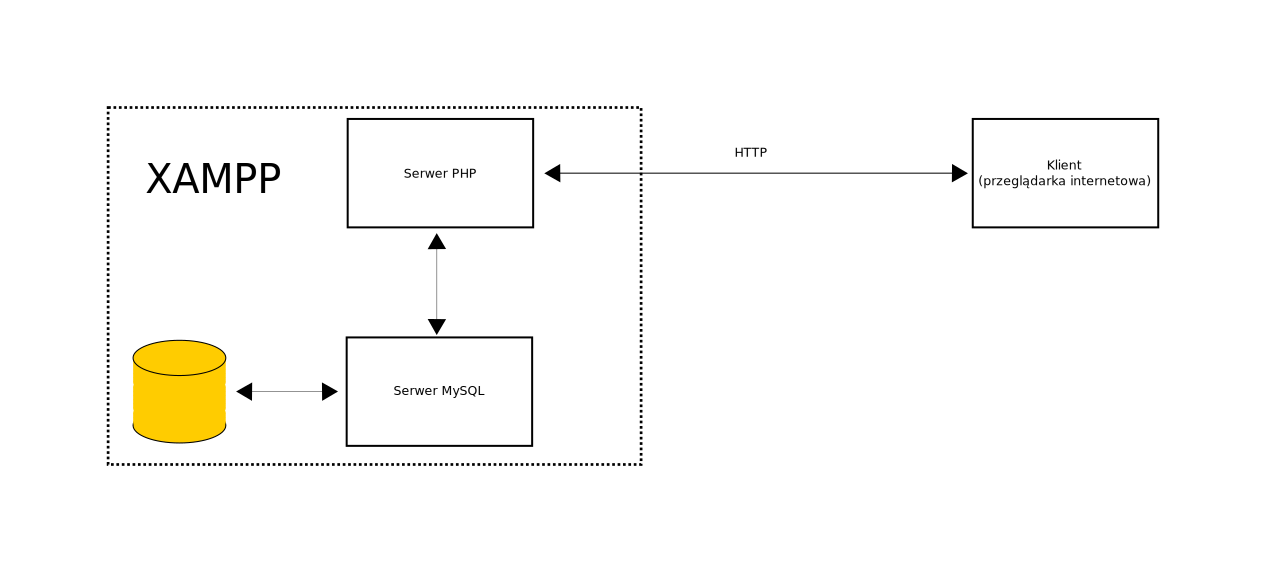
\includegraphics[height=7cm]{schemat.png}
	\caption[Schemat logiczny systemu]{Schemat logiczny systemu}
	\label{fig:schematLogiczny}
\end{figure}

\subsection{Wymagania funkcjonalne}
\subsubsection{Diagram przypadków użycia}
\subsubsection{Scenariusze wybranych przypadków użycia}

\subsection{Wymagania niefunkcjonalne}
\subsubsection{Wykorzystywane technologie i narzędzia}
Technologie:
\begin{itemize}
	\item PHP 7.0
	\item MySQL 5.7.10
	\item HTML 5
	\item CSS 3
	\item LaTeX (dokumentacja)
\end{itemize}
Narzędzia projektowania:
\begin{itemize}
	\item MySQL 5.7.11
	\item MySQL Workbench 6.1
\end{itemize}
Narzędzia implementacji systemu:
\begin{itemize}
	\item GitHub Desktop 3.0.15
	\item NetBeans IDE 8.1
	\item XAMPP 5.6.19
\end{itemize}
\subsubsection{Wymagania dotyczące rozmiaru bazy danych}
\subsubsection{Wymagania dotyczące bezpieczeństwa systemu}
\subsection{Przyjęte założenia projektowe}

\section{Projekt systemu}
\subsection{Projekt bazy danych}
\subsubsection{Analiza rzeczywistości i uproszczony model konceptualny}
\subsubsection{Model logiczny i normalizacja}
\subsubsection{Model fizyczny i ograniczenia integralności danych}
\subsubsection{Inne elementy schematu – mechanizmy przetwarzania danych}
\subsubsection{Projekt mechanizmów bezpieczeństwa na poziomie bazy danych}

\subsection{Projekt aplikacji użytkownika}
\subsubsection{Architektura aplikacji i diagramy projektowe}
\subsubsection{Interfejs graficzny i struktura menu}
\subsubsection{Projekt wybranych funkcji systemu}
\subsubsection{Metoda podłączania do bazy danych – integracja z bazą danych}
\subsubsection{Projekt zabezpieczeń na poziomie aplikacji}

\section{Implementacja systemu}
\subsection{Realizacja bazy danych}
\subsubsection{Tworzenie tabel i definiowanie ograniczeń}
\subsubsection{Implementacja mechanizmów przetwarzania danych}
\subsubsection{Implementacja uprawnień i innych zabezpieczeń}

\subsection{Realizacja elementów aplikacji}
\subsubsection{Obsługa menu}
\subsubsection{Walidacja i filtracja}
\subsubsection{Implementacja interfejsu dostępu do bazy danych}
\subsubsection{Implementacja wybranych funkcjonalności systemu}
\subsubsection{Implementacja mechanizmów bezpieczeństwa}

\section{Testowanie systemu}
\subsection{Instalacja i konfigurowanie systemu}
\subsection{Testowanie opracowanych funkcji systemu}
\subsubsection{Testowanie funkcji 1}
\subsubsection{Testowanie funkcji 2}
\subsection{Testowanie mechanizmów bezpieczeństwa}
\subsection{Inne testy}
\subsection{Wnioski z testów}
\section{Podsumowanie}

\section{Literatura}
\begin{enumerate}[label={[\arabic*]}]
	\item Kierzkowski A., \textit{PHP5. Tworzenie stron WWW}, Helion, Gliwice 2006
	\item http://www.kurshtml.edu.pl/
	\item http://php.net/
	\item http://www.w3schools.com/html/default.asp
	\item http://www.w3schools.com/sql/default.asp
\end{enumerate}
\end{document}